\chapter{Umsetzung}
\label{umsetzungchapter}

In diesem Kapitel soll beschrieben werden, wie die in den vorangegangenen Seiten beschriebene Planung umgesetzt wurde. Dafür wird zuerst erklärt wie eine Technologie ausgewählt wurde, bevor diese dann genauer betrachtet wird. Im Anschluss soll anhand von Beispielen konkret gezeigt werden, wie bestimmte Bausteine implementiert wurden.

Für die Umsetzung des Projektes mussten zu Beginn verschiedene Entscheidungen getroffen werden. Die unterschiedlichen Bausteine des Projektes welche essentiell sind mussten erkannt werden. Anschließend musste entschieden werden, mit welchen Technologien und Arbeitstechniken vorgegangen werden soll. Dafür wurden verschiedene Faktoren berücksichtigt:

\begin{itemize}
\item Wie aufwändig ist eine Umsetzung?
\item Lässt sich das technisch umsetzen?
\end{itemize}

Beide Faktoren und ihr Einfluss sollen kurz erklärt werden.

\paragraph{Aufwand} Der Begriff Aufwand beschreibt verschiedene wichtige Aspekte. Am stärksten wiegt für dieses Projekt der zeitliche Aufwand. Kommt die Frage auf, wie etwas umgesetzt werden soll und nach welchen Methoden gearbeitet werden muss ist es wichtig zu wissen, ob die gewählte Methodik zeitlich realisiert werden kann. Ansonsten scheitert das Projekt. Zeitaufwand wird dabei verursacht durch mangelndes Wissen über Technologie und Arbeitsweise, da dann eine Einarbeitungszeit notwendig wird. Auch ist je nach Technologie ein gewisser Planungsaufwand nötig, um beispielsweise einzelne Elemente in eine passende Form zu gießen.

\newpage

\paragraph{Realisierbarkeit} Da kein Budget investiert werden soll muss mit den Mitteln gearbeitet werden, die gegeben sind. Das gilt sowohl für Hardware als auch Software. Eine Verwendung von exklusiver und teurer Hard-/Software ist deshalb nicht vorgesehen und sollte in der Entscheidung berücksichtigt werden. Unter diesen Aspekt fällt ebenfalls, dass auch der Endnutzer eine gewisse Hardware-Limitation hat. Es kann nicht davon ausgegangen werden, dass jeder einen leistungsfähigen Computer besitzt bzw. bestimmte Software sein Eigen nennt die vielleicht benötigt wird. Deshalb muss die Verwendung von solchen Limitationen unterliegender Technologien vermieden werden.

\section{Verschiedene mögliche Ansätze}

Um die oben genannten Restriktionen einhalten zu können muss jeder Ansatz der als Umsetzungsmethodik in Frage kommt geprüft und bewertet werden. Dies soll im Folgenden näher beschrieben werden:

Der offensichtlichste Ansatz der gewählt werden kann ist der, alles selbst zu programmieren. Das bedeutet, dass jeder einzelne Bestandteil des Projekts mit möglichst viel Handarbeit erstellt wird und nicht auf ein Baukastensystem oder unzählige APIs zurückgegriffen werden soll. Auch wenn es erst so scheint, als bleibe der zeitliche Aufwand gering, da nur eine Sprache gewählt wird und mit der Entwicklung begonnen werden kann, ist das nicht korrekt. Ein genauerer, zweiter Blick zeigt diese Fehleinschätzung deutlich. Ist das Projekt weiter fortgeschritten müssen verschiedene Elemente wie eine Texteingabe oder Codeüberprüfung erstellt werden. Dies lässt sich ohne die Hilfe von APIs nur sehr schwer und zeitaufwändig realisieren. Häufig ist außerdem die eigene Programmierfreiheit durch die feste Wahl auf eine Sprache eingeschränkt, da nicht alle Funktionen ohne weiteres realisiert werden können. Als Beispiel dafür lässt sich die Codeeingabe eines Nutzers heranziehen. Soll ein gut benutzbarer Editor mit Tastenkürzeln und Syntax-Highlighting verwendet werden muss er mit einer API eingebunden werden oder selbst geschrieben sein. Letzteres ist zeitlich nicht zu bewerkstelligen, sodass nur die Alternative einer API bleibt. Schnell ist deshalb klar geworden, dass verschiedene Technologien ein großes Projekt ergeben werden. Allerdings entstehen auch bei diesem Ansatz Nachteile. Nicht jede API oder Technologie ist kompatibel miteinander. Jede hat ihren eigenen Verwendungszweck, so das eine Auswahl getroffen werden muss. Für einen langwierigen Entscheidungsprozess ist jedoch nicht genug Zeit, sodass ein grober Blick ausreichen muss, auch wenn ein Fehlgriff schlechter vermeidbar ist. Der zweite Nachteil, der ebenfalls Grund für eine schnelle Auswahl ist, stellt die Benutzung dar. Nicht immer ist das Wissen darüber vorhanden, sodass erst der Umgang gelernt werden muss. Auch hier muss mit einem großen Zeitaufwand gerechnet werden, der zur Folge hat das nicht sofort mit Ergebnissen gerechnet werden kann. Deshalb sollten zu viele verschiedene Methoden und Technologien genauso vermieden werden wie die Einschränkung auf nur eine einzige. Eine Mischlösung aus beiden Varianten, also einer eigenen Entwicklung mit möglichst wenig Fremdeinwirkung und verschiedene Technologien für verschiedene Bereiche muss gefunden werden.

\section{Unity}

Unity ist ein Framework für Spiele-Entwickler, welches sich durch seine Bekanntheit und Größe auszeichnet. Durch die gezielte Ausrichtung auf das Erstellen von Spielen bietet es sich an, es zur Erstellung eines Educational Games zu verwenden. Viele interne oder durch Plugins nachträglich erzielbare Funktionen können mittels "What You See is What You Get"-Prinzip dazu verwendet werden, fast alle Aufgaben zu erfüllen die benötigt werden. Bereits mit Unity erstelle Projekte zeigen gut, wie komplex es dabei werden kann. Mittels CSharp-Skripten kann eigener Code dazu verwendet werden, nicht ganz so offensichtliche Funktionen zu realisieren. Unity ist dabei am besten mit "leicht zu lernen, schwer zu meistern" zu beschreiben. Simple Spiele sind schnell erstellt, komplexe Aufgaben brauchen jedoch einen erheblich höheren Zeitaufwand. Dadurch wird es einfacher, einen funktionierenden Prototypen zu erstellen. Ob der Aufwand niedriger ist als eine Entwicklung mit einer anderen Herangehensweise kann im Bezug auf eine komplexe Aufgabe nicht aufgezeigt werden. Im Fokus dieser Arbeit steht die Erstellung eines Prototypes, der aufzeigt wie das finale Endprodukt aussehen soll. Dies sollte sich mit Unity realisieren lassen. Dazu wird zuerst die Funktionsweise von Unity betrachtet.

\newpage

\section{Funktionsweise von Unity}

In diesem Abschnitt sollen die kennengelernten Mittel zum Umgang mit Unity beschrieben und erklärt werden. Dabei besteht nicht der Anspruch Unity vollständig zu erklären. Das Ziel hingegen ist, zu zeigen, wie der Grundlegende Aufbau von Unity ist und mit welchen Komponenten und Funktionen im laufe der Erstellung des Prototyps gearbeitet wurde.

\subsection{Die Unity UI}

Unity hat wie jede Entwicklungsumgebung mehrere Fenster mit verschiedenen Funktionen. Die wichtigsten (und am häufigsten genutzten) Fenster sollen im folgenden kurz beschrieben werden:

\begin{itemize}
\item \textit{Project}: Über das Fenster \textit{Project} wird zu den Assets sowie zu anlegbaren Favoriten navigiert. Um den Überblick über die Assets nicht zu verlieren lohnt es sich, sie in einer Ordnerstruktur zu organisieren. Wir haben die Ordner Prefabs, Scenes, Scripts, Sounds, Sprites und Textures angelegt. Deren Inhalt wird im laufe des Abschnittes noch erläutert werden.
\item \textit{Hierarchy}: In diesem Fenster werden alle Elemente/Objekte einer geladenen Szene hierarchisch nach ihren Abhängigkeiten mit Namen angezeigt. Bei einem Klick auf ein Objekt, wird dieses in dem Fenster \textit{Scene} markiert.
\item \textit{Scene} und \textit{Game}: Im Fenster \textit{Scene} kann der aktuelle Stand des Spiels, beziehungsweise der geladenen Szene, eingesehen werden. Das bedeutet, dass alle Objekte der Szene anklickbar sind und daraufhin im \textit{Inspector} Fenster untersucht werden können. Per Drag and Drop können der Szene weitere Elemente aus der \textit{Project} Übersicht hinzugefügt werden.
Wenn auf den Play Button (oben in der Mitte der UI von Unity) gedrückt wird, wechselt Unity automatisch in das \textit{Game} Fenster und die aktuelle Szene kann als \glqq echtes \grqq Spiel getestet werden.  \newpage
\item \textit{Inspector}: Wird ein Objekt in dem Fenster \textit{Scene} oder aus der \textit{Hierarchy} ausgewählt, können weitere Informationen zu dem Objekt in diesem Fenster eingesehen und verändert werden. Zum Beispiel Größe, Position, Farbe und Verhalten. Letzteres kann durch Verknüpfen eines Scripts mit diesem Objekt realisiert werden. 
\item \textit{Console}: In diesem Fenster werden alle Texte und Fehlermeldungen ausgegeben.
\end{itemize}

\subsection{Was für Elemente verwendet werden können}
\label{Elemente}

Um das Spiel mit Unity zu gestalten, gibt es verschiedene Elemente, die verwendet werden können. 

\subsubsection{Szene}

Den grundlegenden Baustein stellt dabei die Szene dar. Diese enthalten die verschiedenen Umgebungen und Menüs des Spiels, wobei jede Szene als eigenes Level gesehen werden kann. Auf einer Szene können verschiedenen \textit{GameObjects} angeordnet werden. Per C\# Skript (siehe Beispiel in Abschnitt \ref{u_beispiele}) kann zwischen den verschiedenen Szenen gewechselt werden. Doch was sind eigentlich die mehrfach genannten Game Objekte? ~\cite{F_6.3.2.1_Scenes}

\subsubsection{Game Objekt}
Das Game Objekt ist das wichtigste Konzept in der Gestaltung von Szenen. Jedem Objekt des Spiels liegt ein Game Objekt zu Grunde. Allerdings kann ein leeres Game Objekt nichts alleine tun. Um ihm eine besondere Bedeutung oder Verhalten zu geben, muss dem Game Objekt eine oder mehrere Komponenten (je nach Objekttyp welcher erstellt werden soll) hinzugefügt werden. Ein Game Objekt kann zum Beisiel in der Hierarchie per Rechtsklick erstellt werden. Hier gibt es die Möglichkeit ein leeres Game Objekt zu erstellen, oder schon vorgefertigte Objekte zu verwenden. Ist es erstellt können dem Objekt Komponenten hinzugefügt werden, damit es zu dem werden kann, zu dem es bestimmt ist. Die Komponente \textit{Transform} muss in jedem Game Objekt enthalten sein. Deswegen wird sie automatisch zu einem neu erstellten Objekt hinzugefügt und kann auch nicht gelöscht werden. Die Komponente legt Position und Ausrichtung fest. ~\cite{F_6.3.2.2_GameObjekts}

\subsubsection{Komponenten}
Komponenten sind zum Beispiel Effekte, Licht, Text, Formen, Ton, Video oder Skripte. Mit Hilfe der Skripting API können auch eigene Komponenten erstellt werden. Komponenten stellen, wie oben schon angedeutet, die eigentliche Funktionalität von Game Objekten. Zum Beispiel enthält jede erzeugte Szene von Beginn an das Main Camera Game Objekt. Dieses \glqq normale\grqq Game Objekt wird durch die hinzugefügte Komponente \textit{Camera Component} erst zur Kamera, durch die der Spieler die Spielwelt sehen kann.

Es gibt mehrere Möglichkeiten um eine Komponente zu einem Game Objekt hinzuzufügen. Zum einen über das Component Menü in der Werkzeugleiste, oder insofern das Objekt gerade ausgewählt ist, über den Inspektor und die Schaltfläche \textit{Add Component}. 

Eine Komponente mehrere Properties besitzen. Diese sind entweder vom Typ \textit{value} oder \textit{reference}. Values sind einfache Werte, welche direkt im Inspektor angepasst aber auch im laufenden Spiel über eigene Skripte verändert werden können. References stellen Verweise auf jegliche Art von Game Objekten dar. Diese können einfach per Drag and Drop hinzugefügt werden.

Unity bietet eine sehr gute Dokumentation über die verschiedenen Komponenten. Die jeweilige \textit{Component Reference Page} ist auch über das Fragezeichen-Symbol im Inspector neben dem Komponentennamen erreichbar. \cite{F_6.3.2.3_Komponenten}

\subsubsection{Assets und Prefabs}
Ein Asset ist eine Repräsentation von irgendeinem Item, welches im Unity Projekt verwendet werden kann, sozusagen der Überbegriff.

Prefabs sind ein Asset Typ, der es dem Entwickler erlaubt, Game Objekte komplett mit allen Komponenten und Skripten als eine \glqq Vorlage \grqq zu speichern. Das ist besonders dann hilfreich, wenn das Game Objekt sehr oft verwendet werden soll. Denn ein Prefab hat den Vorteil (vor normalem Copy/Paste), dass wenn das Prefab verändert werden sollte, alle Instanzen die davon in der Spiele Welt existieren entsprechend mit verändert werden. ~\cite{F_6.3.2.4_Prefabs} 

\subsubsection{Sprites}

Sprites sind einfache graphische 2D Objekte, also Bilder, welche einem Game Objekt zugeordnet werden können. ~\cite{F_6.3.2.5_Sprites}

\subsubsection{Skripte}
Möchte der Entwickler einem Game Objekt Funktionalität geben, welche sich noch nicht in vordefinierten Komponenten findet, hat er die Möglichkeit diese in Form von einem Skript selbst zu definieren. Unity unterstützt zwei verschiedene Sprachen: C\# und UnityScript. Durch Skripte können beispielsweise Game Events getriggert werden, Komponenten Properties während der Laufzeit des Spiels verändern und auf Nutzereingaben reagieren. ~\cite{F_6.3.2.6_Skripte}

Ein Script kann wie jede andere Komponente ebenfalls über den \textit{Add Component} Button im Inspektor hinzugefügt werden. Sollte es sich bei dem Game Objekt um ein anklickbares Objekt handeln, kann im Inspektor ebenfalls definiert werden, welches Skript und welche Methode aus dem Skript als Folge eines Klicks ausgeführt werden sollen.

In Abschnitt \ref{u_beispiele} wird auf den Aufbau und die Funktion der Skripte noch näher eingegangen.


\subsection{Zusammenarbeit}
Da dieses Projekt zu zweit entwickelt wird, stellte sich natürlich auch die Frage, wie der Code geteilt und versioniert werden kann. Eine Verwendung von GitHub, einer Plattform die genau diese Aufgabe erfüllt, wurde kurz nachgedacht. Da dazu aber die Verwendung von Add-ons und diverse Einstellungen nötig waren wurde aufgrund der einfachen Handhabung und des geringen Konfigurationsaufwandes eine zweckmäßige Alternative gesucht. Diese fand sich in Unity selbst, denn genau für die Frage der Teamzusammenarbeit bietet Unity von Haus aus die Funktion Collaborate an. Auf der Homepage wird die Funktion wie folgt beschrieben: \glqq Collaborate ist ein einfacher Weg für Teams, ihr Unity-Projekt zu speichern, zu teilen und zu synchronisieren. Collaborate ist Cloud-gehostet und benutzerfreundlich, sodass das gesamte Team zum Projekt beitragen kann, unabhängig von Standort und Rolle. \grqq ~\cite{F_6.3_UnityCollab} 

\section{Beispielhafte Implementierung einer Funktion in Unity}
\label{u_beispiele}
In diesem Abschnitt werden einige Beispiele aus dem Projekt in Form von Code und Erklärungen gezeigt, um einen Überblick über die Implementierung zu geben, sowie die Handhabung von Unity und der Scripting API aufzuzeigen.

\subsection{Beispielhalfter Aufbau eines Skripts}
Listing \ref{lst:BeispielSkript} zeigt ein in Unity neu erstelltes Skript mit dem Namen \textit{BeispielSkript}. Gut zu erkennen ist, dass der Klassennamen immer dem Skriptnamen entsprechen muss, damit das Skript als Komponente an ein Game Objekt gebunden werden kann. Jedes Skript muss die Klasse \textit{Monobehaviour} implementieren, wenn eine Verbindung zu den inneren Funktionen von Unity aufgebaut werden soll.

Per Default hat ein Skript zwei Funktionen. Diese können, müssen aber nicht verwendet werden. Die Funktion \textit{Start()} wird aufgerufen, bevor das Spiel beginnt. Da in Unity Objekte nicht durch einen selbstdefinierten Konstruktor erstellt werden, sondern von Unity selbst, ist stattdessen hier der Platz um nötige Initialisierungen durchzuführen. In der Funktion \textit{Update()} können Aktionen abgehandelt werden, die während dem Spielen auftreten, wie zum Beispiel Benutzereingaben oder eine Bewegung des Spielers.

\lstset{style=sharpc}
\begin{lstlisting}[caption=Beispiel Skript, label=lst:BeispielSkript]

using System.Collections;
using System.Collections.Generic;
using UnityEngine;

public class BeispielSkript : MonoBehaviour {

	// Use this for initialization
	void Start () {		
	}	
	// Update is called once per frame
	void Update () {	
	}
}
\end{lstlisting}

\subsection{Szenenwechsel}
Wie in Abschnitt \ref{Elemente} beschrieben, sind Szenen wichtige grundlegende Bausteine für die Erstellung eines Spiels. Da ein Spiel nicht nur aus einer Szene besteht, sondern aus einer Vielzahl dieser, sollte es die Möglichkeit geben, zwischen den verschiedenen Szenen wechseln zu können. Hierfür bietet die Unity Scripting API eine einfache Funktion:

\lstset{style=sharpc}
\begin{lstlisting}[caption=Szenenwechsel, label=lst:Szenenwechsel]

public class LoadSceneOnClick : MonoBehaviour {
	
    public void LoadByIndex(int sceneIndex) {
        SceneManager.LoadScene(sceneIndex);
    }
}

\end{lstlisting}

In Listing \ref{lst:Szenenwechsel} ist die selbstgeschriebene Funktion \textit{LoadByIndex} für den Szenenwechsel zu sehen. Hierfür wurde die Methode \textit{LoadScene(sceneIndex)} des SceneManagers verwendet. Ruft ein Game Objekt oder ein anderes Skript die eigene Methode des Skripts \textit{LoadSceneOnClick} auf, wird zu der Szene mit dem angegebenen Index gewechselt. 

Welche Szene welchen Index besitzt, kann in den Build Settings festgelegt werden (Abbildung \ref{BuildSettingsPic}). Hier müssen alle Szenen, welche verwendet werden sollen, eingetragen werden. Jede neue Szene erhält dabei einen eindeutigen Index. Durch anklicken und ziehen einer Szene kann die Reihenfolge und damit auch der Index verändert werden. Der beim Hinzufügen einer Szene angelegte Index ist also nicht endgültig.

\begin{figure}
\centering
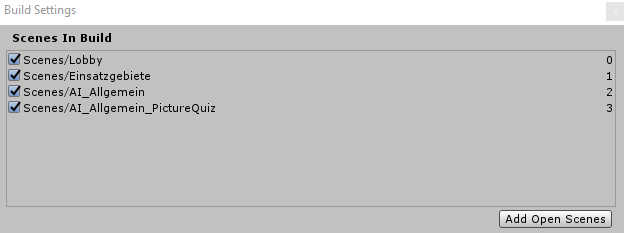
\includegraphics[scale=0.85]{bilder/BuildSettings.PNG}
\caption{Build Settings}
\label{BuildSettingsPic}
\end{figure}

\subsection{Die Lobby}

\subsection{Ein Quiz}
In diesem Abschnitt wird etwas ausführlicher beschrieben, wie ein Quiz implementiert werden kann. Er stellt nicht den Anspruch, die einzig richtige Art und Weise zu sein, wie das möglich ist. Damit am Ende nicht nur eine unbewegliche Oberfläche heraus kommt, braucht es zusätzlich zu dieser noch ein paar Skripte und das EventSystem (vorgefertigtes Game Objekt), welches für die Verarbeitung von Events in der Unity Szene zuständig ist. Sonst existiert in der Quizszene nur noch die \textit{Default Kamera}, welche aber unverändert bestehen bleiben kann.

\subsubsection{Die Oberfläche}
Alle Elemente der Oberfläche werden auf dem sogenannten Canvas angeordnet. Dieser dient wie in Java Swing ein Frame als Container für alle weiteren Game Objekte. In Abbildung \ref{QuizOberflaechePc} ist die Quizoberfläche im Szenenfenster zu sehen. Das Canvas ist durch die vier blauen Punkte an den Ecken gekennzeichnet. (Hinweis: So sieht es im Szenenfenster immer aus, wenn ein Element in der Hierarchie oder direkt in der Szene selektiert wurde). Die sechs hellen Rechtecke sind Button, denen jeweils ein Text zugeordnet wurde. Die beiden dunklen Bereiche sind Panel, denen ebenfalls ein Text zugeordnet wurde. 

Wie die gesamte Szene aufgebaut ist, kann im Fenster Hierarchie gesehen werden (Abbildung \ref{HierarchiePc}). Eine weitere Komponente, welche bisher verschwiegen wurde, ist der GameManager. Dieser ist ganz oben in der Hierarchie zu sehen und stellt einfach ein leeres Game Objekt dar, welches mit dem in Abschnitt \ref{QuizSkripte} erklärten GameManager-Skript verknüpft wird. Sobald alle Funktionen implementiert sind, können über dieses Game Objekt die verschiedenen Fragen und die dazugehörigen Antworten im Inspektor eingegeben werden. Auch die Verknüpfung zwischen den im Skript definierten Variablen und den UI Komponenten findet in diesem Game Objekt statt.

\begin{figure}
\centering
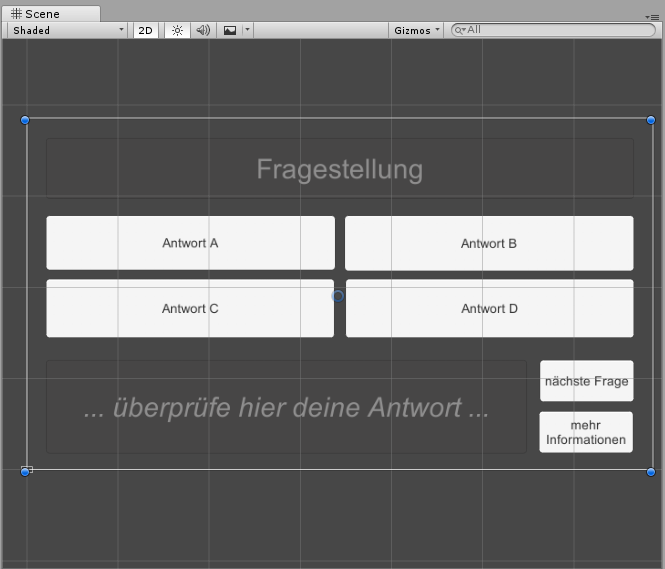
\includegraphics[scale=0.8]{bilder/QuizOberflaecheSzene.PNG}
\caption{Die Quiz Oberfläche im Szenen Fenster}
\label{QuizOberflaechePc}
\end{figure}

\begin{figure}
\centering
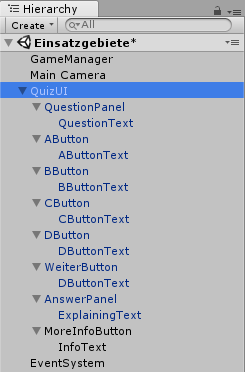
\includegraphics[scale=1]{bilder/Hierarchie.PNG}
\caption{Hierarchie}
\label{HierarchiePc}
\end{figure}

\subsubsection{Die Skripte}
\label{QuizSkripte}
Damit die Buttons und die Panel auch mit Funktionen belegt sind, müssen diese mit Skripten verbunden werden, sonst bleibt unsere UI unbeweglich und somit nicht spielbar.

Zwei Skripte sind essentiell. Das Skript \textit{Question} ist lediglich ein Model, über welches später aus dem \textit{GameManager-Skript} auf die verschieden Fragen und Antwortet zugegriffen werden soll. Deshalb weicht der Aufbau des C\# Skriptes auch leicht von der vorgestellten Art und Weise ab. 

Etwas komplexer ist das Skript für den GameManager. Neben sieben verschiedene Funktionen um dem Quiz seine \glqq Seele\grqq zu geben gibt es einigen Variablen- und Komponentendeklarationen. Variablen halten zum Beispiel die aktuelle Frage oder ein Array aller Fragen. Mit Komponentendeklarationen sind variablen gemeint, die auf eine Komponente innerhalb der UI verweisen. Zum Beispiel kann der Button für weitere Informationen oder der Text des Antwortpanels mit dem Code aus Listing \ref{lst:ButtonMoreInformation} angesprochen und kontrolliert werden.

\lstset{style=sharpc}
\begin{lstlisting}[caption=Deklaration von UI Komponenten, label=lst:ButtonMoreInformation]
[SerializeField]
private Button moreInfoButton;

[SerializeField]
private Text answerText;
\end{lstlisting}

Das allgemeine Prinzip ist, dass zunächst alle vorhandenen Fragen aus dem GameManager in ein Array geladen werden. Um das doppelte stellen von Fragen zu vermeiden wird eine Liste von ungefragten Fragen angelegt, welche beim Start gefüllt wird. Wurde eine Frage richtig beantwortet, kann diese aus der Liste gelöscht werden.

Folgende Aufzählung gibt einen kurzen Überblick, welche Funktionen das Skript enthält:

\begin{itemize}
\item Start(): Füllen der Variablen mit den Frage/Antworten aus dem GameManager Objekt und Vorbereiten der UI Komponenten
\item SetCurrentQuestion(): Eine Frage aus den unbeantworteten Fragen auswählen, als aktuelle Frage festlegen und auf der UI anzeigen. Wird von Start() aufgerufen. Ruft seinerseits SetButtonText() auf.
\item SetButtontext(): Belegt die Button mit den jeweiligen Antwortmöglichkeiten.
\item TransitionToNextQuestion(): Wird aufgerufen wenn der Button \glqq nächste Frage \grqq geklickt wird. Wenn noch Fragen vorhanden sind, wird die nächste Frage geladen, wenn nicht, dann wird zur nächsten Szene gewechselt.
\item ShowMoreInformation(): Wird aufgerufen wenn der Button \glqq mehr Informationen \grqq geklickt wird. Zeigt den in der Frage hinterlegten Text mit weiteren Informationen auf der Oberfläche an.
\item DisableMoreInformationButtonIfNull(): Sollten keine weiteren Informationen vorhanden sein, wird der Button disabled. Wird von der Funktion UserSelectQuestion() aufgerufen.
\item UserSelectQuestion(): Diese Funktion prüft, ob der Nutzer die richtige Antwort ausgewählt hat.
\end{itemize}

Um das Zusammenspiel von UI Komponenten und Skript zu verdeutlichen, wird im Folgenden die Funktion ShowMoreInformation() (Listing \ref{lst:ShowMoreInformation}) genauer betrachtet.

\lstset{style=sharpc}
\begin{lstlisting}[caption=Verwendung von UI Komponenten im Skript, label=lst:ShowMoreInformation]
public void ShowMoreInformation()
{
    string moreInformationText = currentQuestion.moreInformation;
    answerText.color = Color.cyan;
    answerText.fontSize = 14;      
    answerText.text = moreInformationText;
}
\end{lstlisting}

Zunächst wird der Informationstext aus der aktuellen Frage ausgelesen und in die Variable \textit{moreInformationText} geschrieben. Die zwei Zeilen darauf sind für Farbe und Schriftgröße zuständig. In der letzten Zeile wird nun noch der Inhalt dem Textfeld zugewiesen.

Wie oben schon beschrieben, wird die Funktion durch den Klick des Buttons ausgelöst. Dies wird dadurch erreicht, dass dem Button im Inspektor diese Funktion hinzugefügt wird. Da das Game Objekt ein Button ist, enthält er im Inspektor das Feld onClick(). Hier kann wie in Abbildung \ref{onClickPc} zu sehen, zunächst ein Skript hinzugefügt und anschließend daran eine Funktion aus dem Skript ausgewählt werden (in diesem Fall die Funktion ShowMoreInformation()).

\begin{figure}
\centering
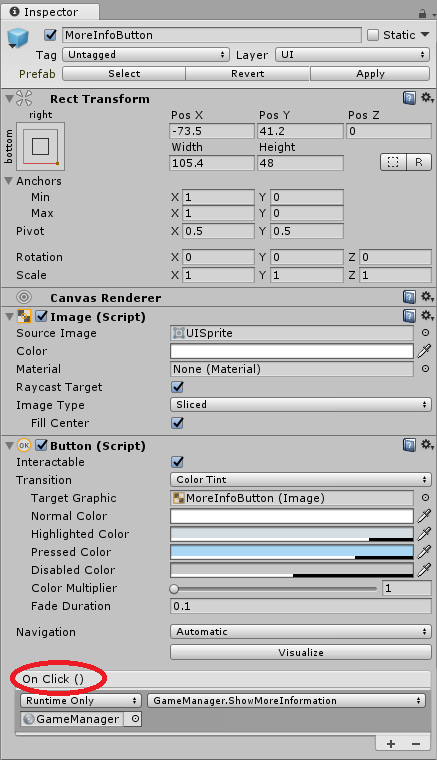
\includegraphics[scale=0.9]{bilder/OnClick2.PNG}
\caption{onClick() Methode im Button}
\label{onClickPc}
\end{figure}
